% CVPR 2023 Paper Template
% based on the CVPR template provided by Ming-Ming Cheng (https://github.com/MCG-NKU/CVPR_Template)
% modified and extended by Stefan Roth (stefan.roth@NOSPAMtu-darmstadt.de)

\documentclass[10pt,twocolumn,letterpaper]{article}

%%%%%%%%% PAPER TYPE  - PLEASE UPDATE FOR FINAL VERSION
\usepackage[review]{cvpr}      % To produce the REVIEW version
%\usepackage{cvpr}              % To produce the CAMERA-READY version
%\usepackage[pagenumbers]{cvpr} % To force page numbers, e.g. for an arXiv version

% Include other packages here, before hyperref.
\usepackage{graphicx}
\usepackage{amsmath}
\usepackage{amssymb}
\usepackage{booktabs}
\usepackage{multirow}
\usepackage{multicol}

% It is strongly recommended to use hyperref, especially for the review version.
% hyperref with option pagebackref eases the reviewers' job.
% Please disable hyperref *only* if you encounter grave issues, e.g. with the
% file validation for the camera-ready version.
%
% If you comment hyperref and then uncomment it, you should delete
% ReviewTempalte.aux before re-running LaTeX.
% (Or just hit 'q' on the first LaTeX run, let it finish, and you
%  should be clear).
\usepackage[pagebackref,breaklinks,colorlinks]{hyperref}


% Support for easy cross-referencing
\usepackage[capitalize]{cleveref}
\crefname{section}{Sec.}{Secs.}
\Crefname{section}{Section}{Sections}
\Crefname{table}{Table}{Tables}
\crefname{table}{Tab.}{Tabs.}


%%%%%%%%% PAPER ID  - PLEASE UPDATE
\def\cvprPaperID{*****} % *** Enter the CVPR Paper ID here
\def\confName{CVPR}
\def\confYear{2023}


\begin{document}

%%%%%%%%% TITLE - PLEASE UPDATE
\title{Expand Big, Then Shrink: An Automatic Way to Generating Efficient Super Resolution Model}


\author{Daheng Yin, Mengyang Liu, Baijun Chen, Fang Dong\\
School of Computer Science and Engineering, Southeast University, Nanjing, China\\
{\tt\small \{yindaheng98, myliu, bjchen, fdong\}@seu.edu.cn}
}
\maketitle

%%%%%%%%% ABSTRACT
\begin{abstract}
  Super-resolution techniques have become increasingly popular in recent years due to their ability to generate high-resolution images from low-resolution counterparts, which is an ill-posed problem in computer vision. Deep convolutional neural networks have shown exceptional performance in Single Image Super-Resolution (SISR), leading to the development of numerous deep learning-based methods. However, with mobile devices becoming a ubiquitous part of everyday life, there is a growing interest in developing Efficient Image Super-Resolution (EISR) methods that are computationally efficient and can produce high-quality images on mobile devices. This paper proposes a model-scaling based method to design an efficient model structure automatically. The "Expand Big, Then Shrink" method expands an old SOTA model to a new, larger dataset and then shrinks it, resulting in a more efficient model structure.
  Our proposed method demonstrates improved performance in terms of FLOPs reduction and PSNR scores compared to existing methods. We get 4.3\% and 8.9\% improvement of PSNR and SSIM respectively. Our approach achieved a low average test and validation time of 40.84ms.
  The study's contributions include a discussion of how to design an efficient model in an automatic way, the proposed method to adapt an old SOTA model to a new, bigger dataset, and evaluation of the method on mainstream datasets.
\end{abstract}

%%%%%%%%% BODY TEXT
\section{Introduction}
\label{sec:intro}

Single Image Super-Resolution (SISR) aims to reconstruct high-resolution images from their low-resolution counterparts, which is an ill-posed problem in computer vision. Over the years, deep convolutional neural networks have demonstrated remarkable performance in this domain, leading to the development of many deep learning-based methods. SISR has found widespread applications, including video gaming and video streaming, where high-resolution displays with high refresh rates are crucial. In particular, mobile devices have benefited from SISR techniques to enhance the user experience. However, mobile phones' power-constrained design with a limited power supply has made Efficient Image Super-Resolution (EISR) a topic of growing interest. Therefore, there is a need to explore EISR methods that are computationally efficient and can produce high-quality images on mobile devices.

Designing an efficient model is non-trivial and always tedious. On one hand, lots of existing work look for insights for reducing FLOPs on operations but which always ignores realistic execution on chip. On the other hand, the macro architecture design of model is also important such as using multiple connections, multiple resolutions, and local sharing. The space to design a SOTA model is too large and it's always fatiguing to update model with complex design over and over.

In this paper, we proposed a model-scaling based method to generate a more efficient model structure by an automatic procedure: first expanding and then shrinking.\ref{fig:overview}

% TODO: 写一段结果
Our proposed method demonstrates superior performance in terms of reducing the number of floating-point operations (FLOPs) and improving the peak signal-to-noise ratio (PSNR) scores compared to existing methods. Specifically, our approach shows a 4.3\% improvement in PSNR and an 8.9\% improvement in structural similarity index (SSIM). Furthermore, our method achieves a low average testing and validation time of 40.84ms.

The main contributions of this work are as follows:

\begin{itemize}
    \item Discussing on how to design an efficient model in an automatic way.
    \item Proposing \"Expand Big, Then Shrink\" method to automatic adapting an old SOTA model to a new bigger dataset which is an efficient way to design new model.
    \item Evaluating our method on main stream datasets and compared our results with other peers in NTIRE-ESRX4 challenge.
\end{itemize}

\begin{figure}[t]
  \centering
  % \fbox{\rule{0pt}{2in} \rule{0.9\linewidth}{0pt}}
   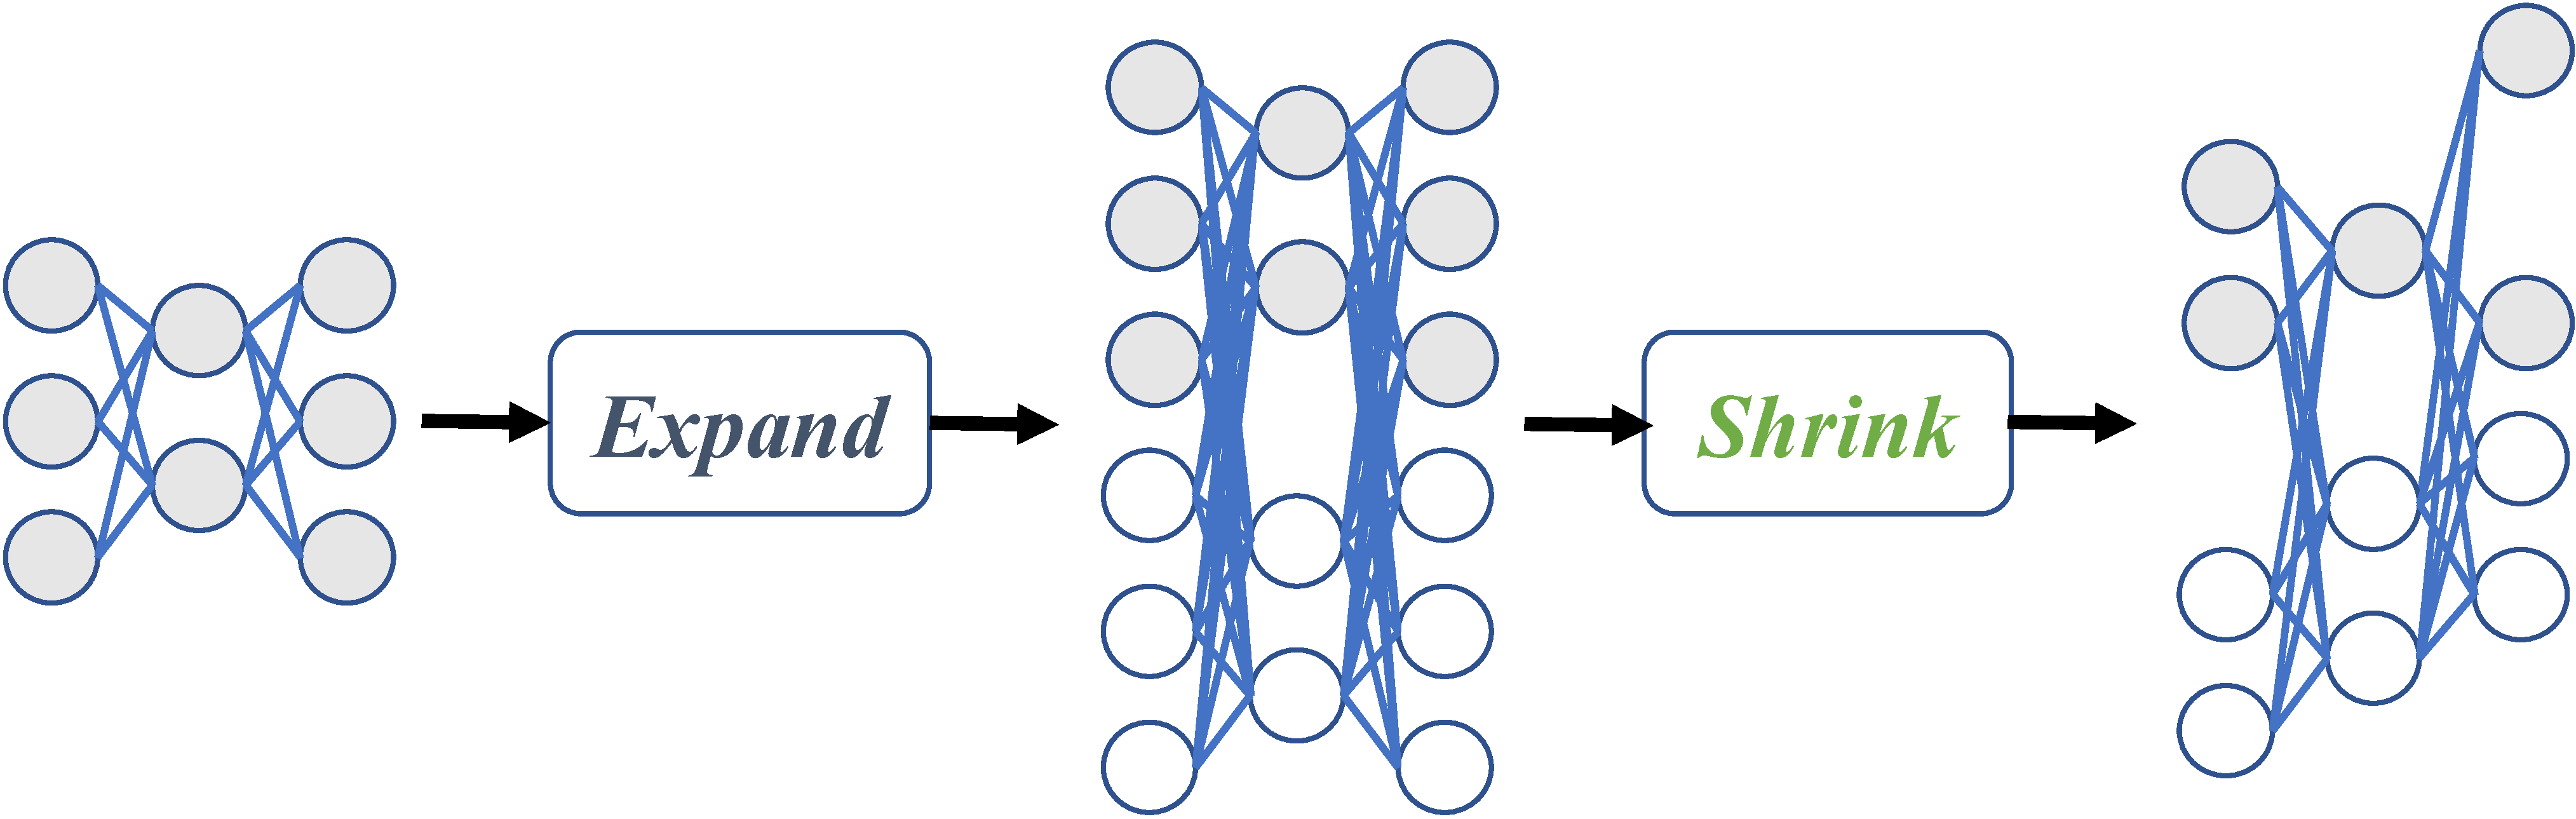
\includegraphics[width=0.8\linewidth]{../expandandshrink.pdf}

   \caption{Designing and training a SOTA model is a non-trivial work. Our work shows that expanding an existing model and then shrink it by pruning and finetuning is an efficient way to improve the performance of model.}
   \label{fig:overview}
\end{figure}



%------------------------------------------------------------------------
\section{Related Work}
\label{sec:related}

Related work.


%------------------------------------------------------------------------
\section{Method}
\label{sec:method}

\begin{figure*}
    \centering
    \begin{subfigure}[b]{0.49\linewidth}
		\centering
        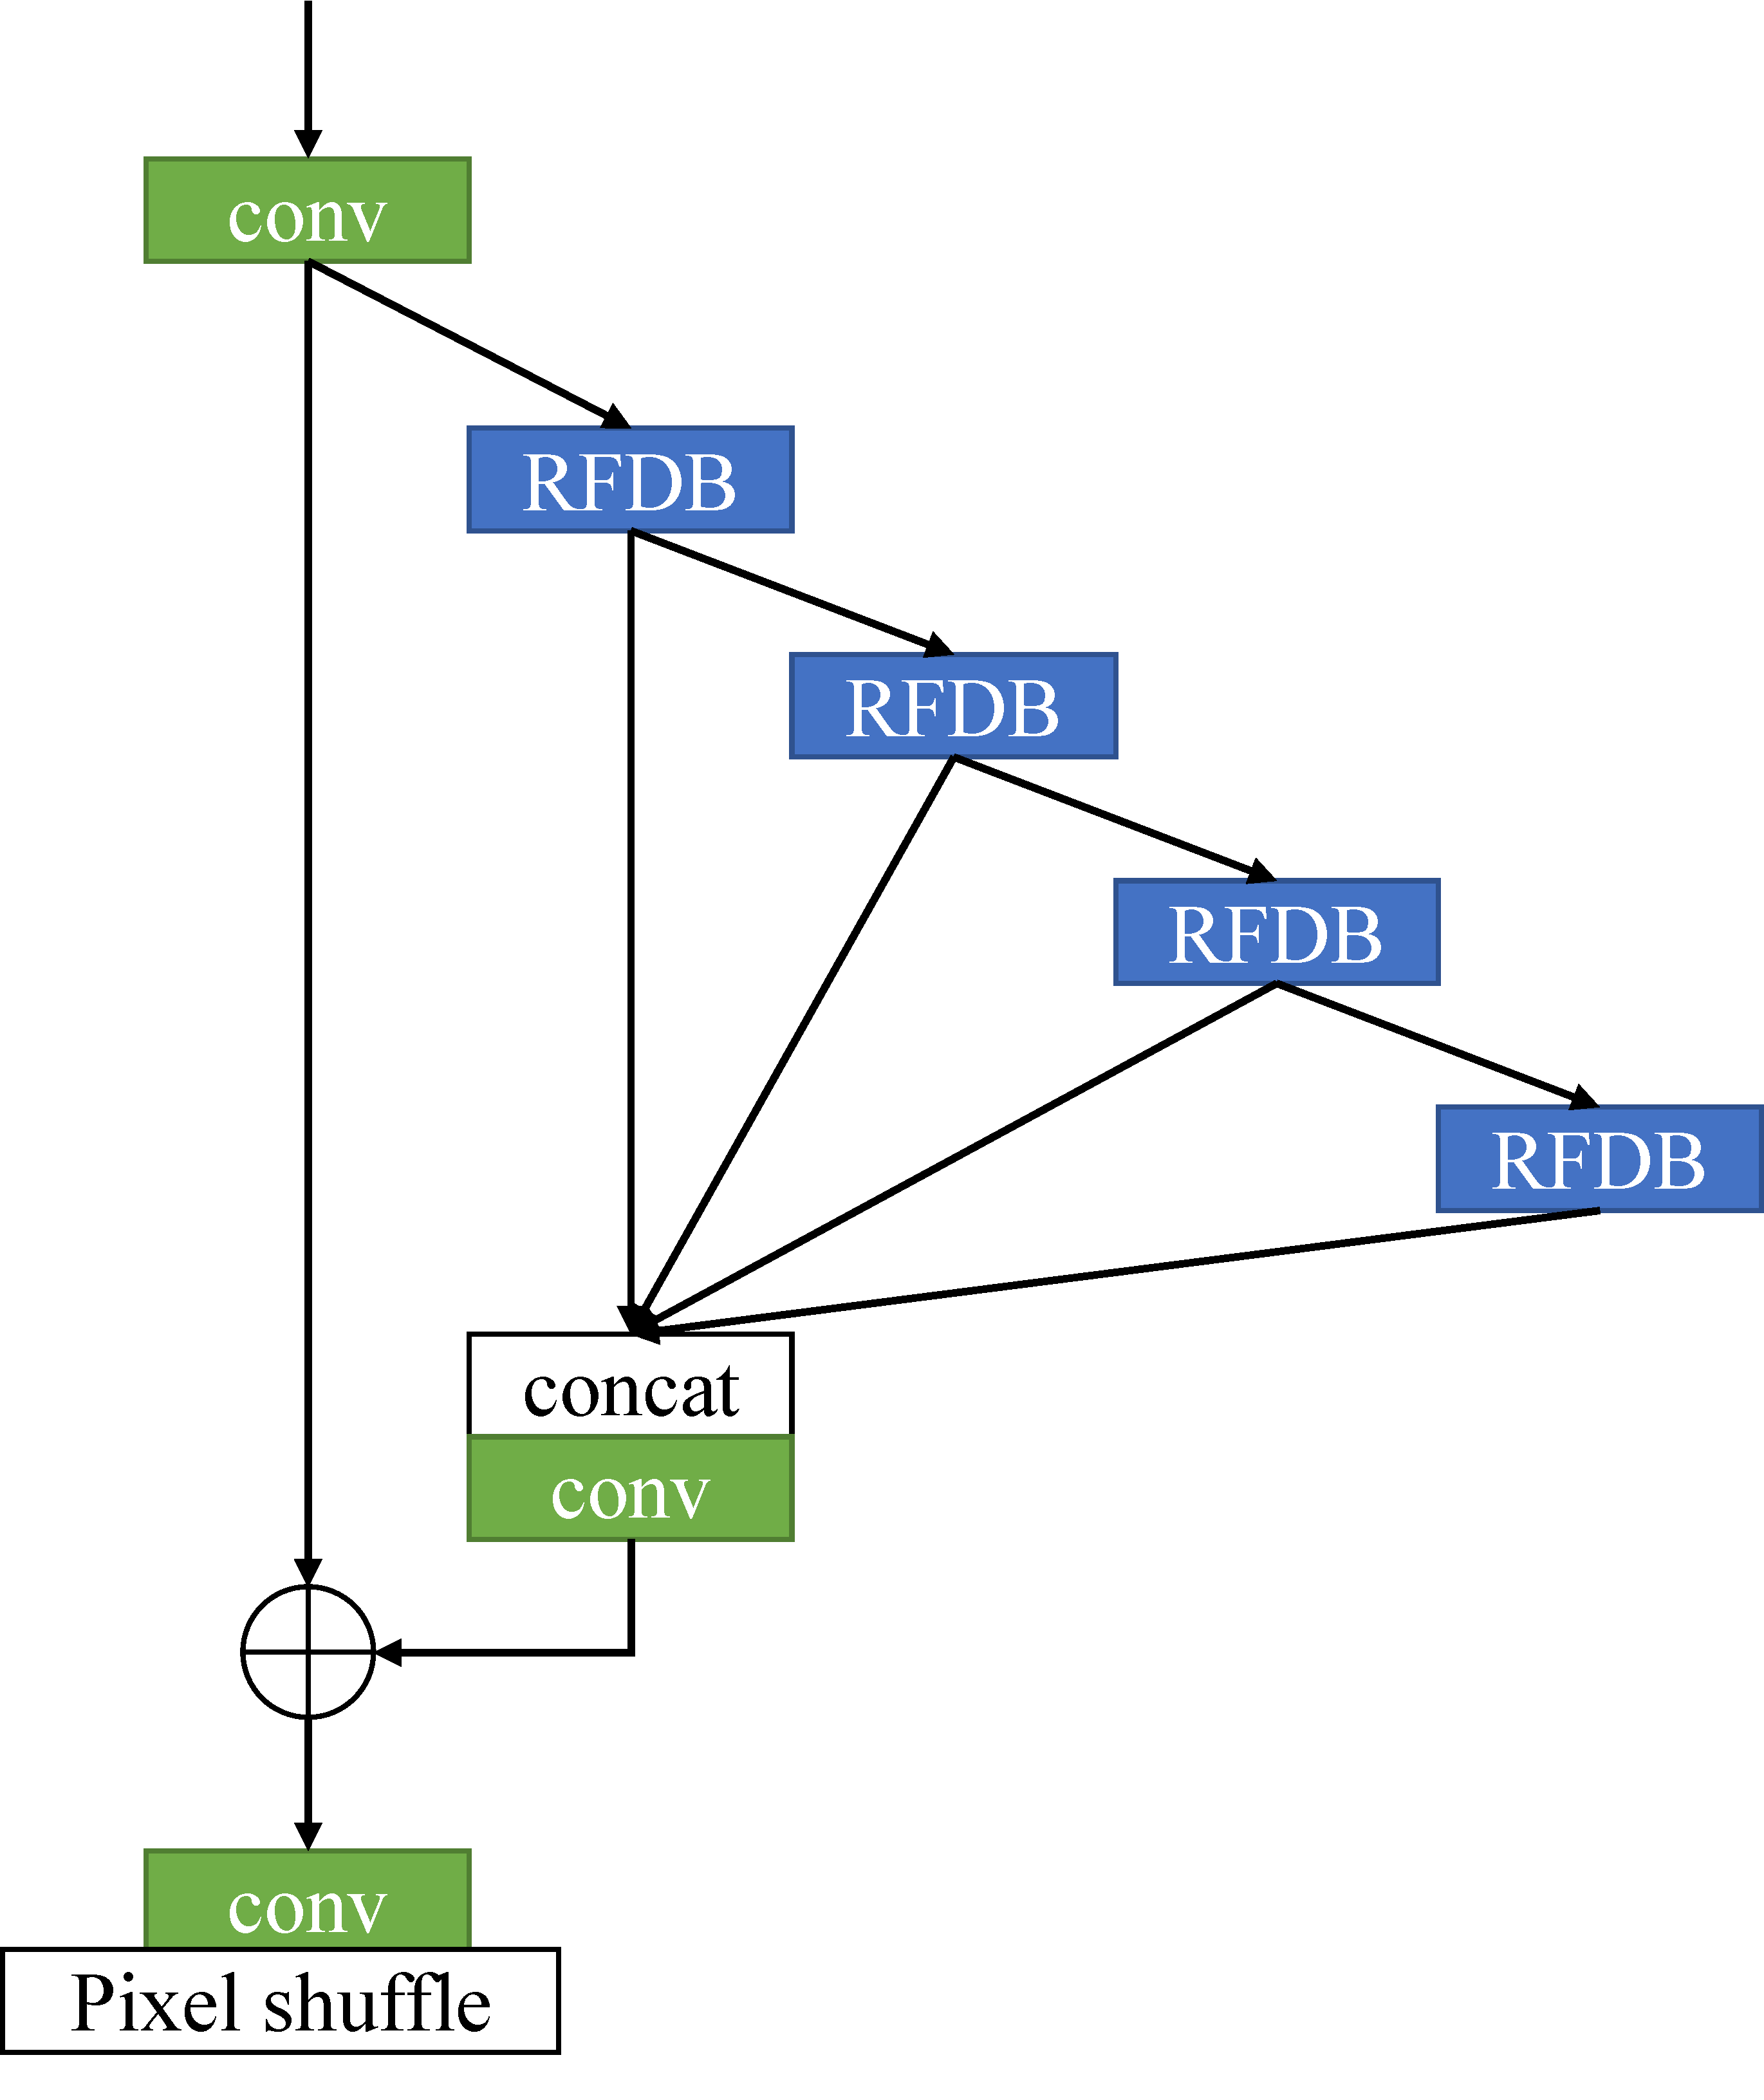
\includegraphics[width=\textwidth]{../RFDN.pdf}
        \caption{RFDN}
        \label{fig:RFDN}
    \end{subfigure}
    \begin{subfigure}[b]{0.49\linewidth}
		\centering
        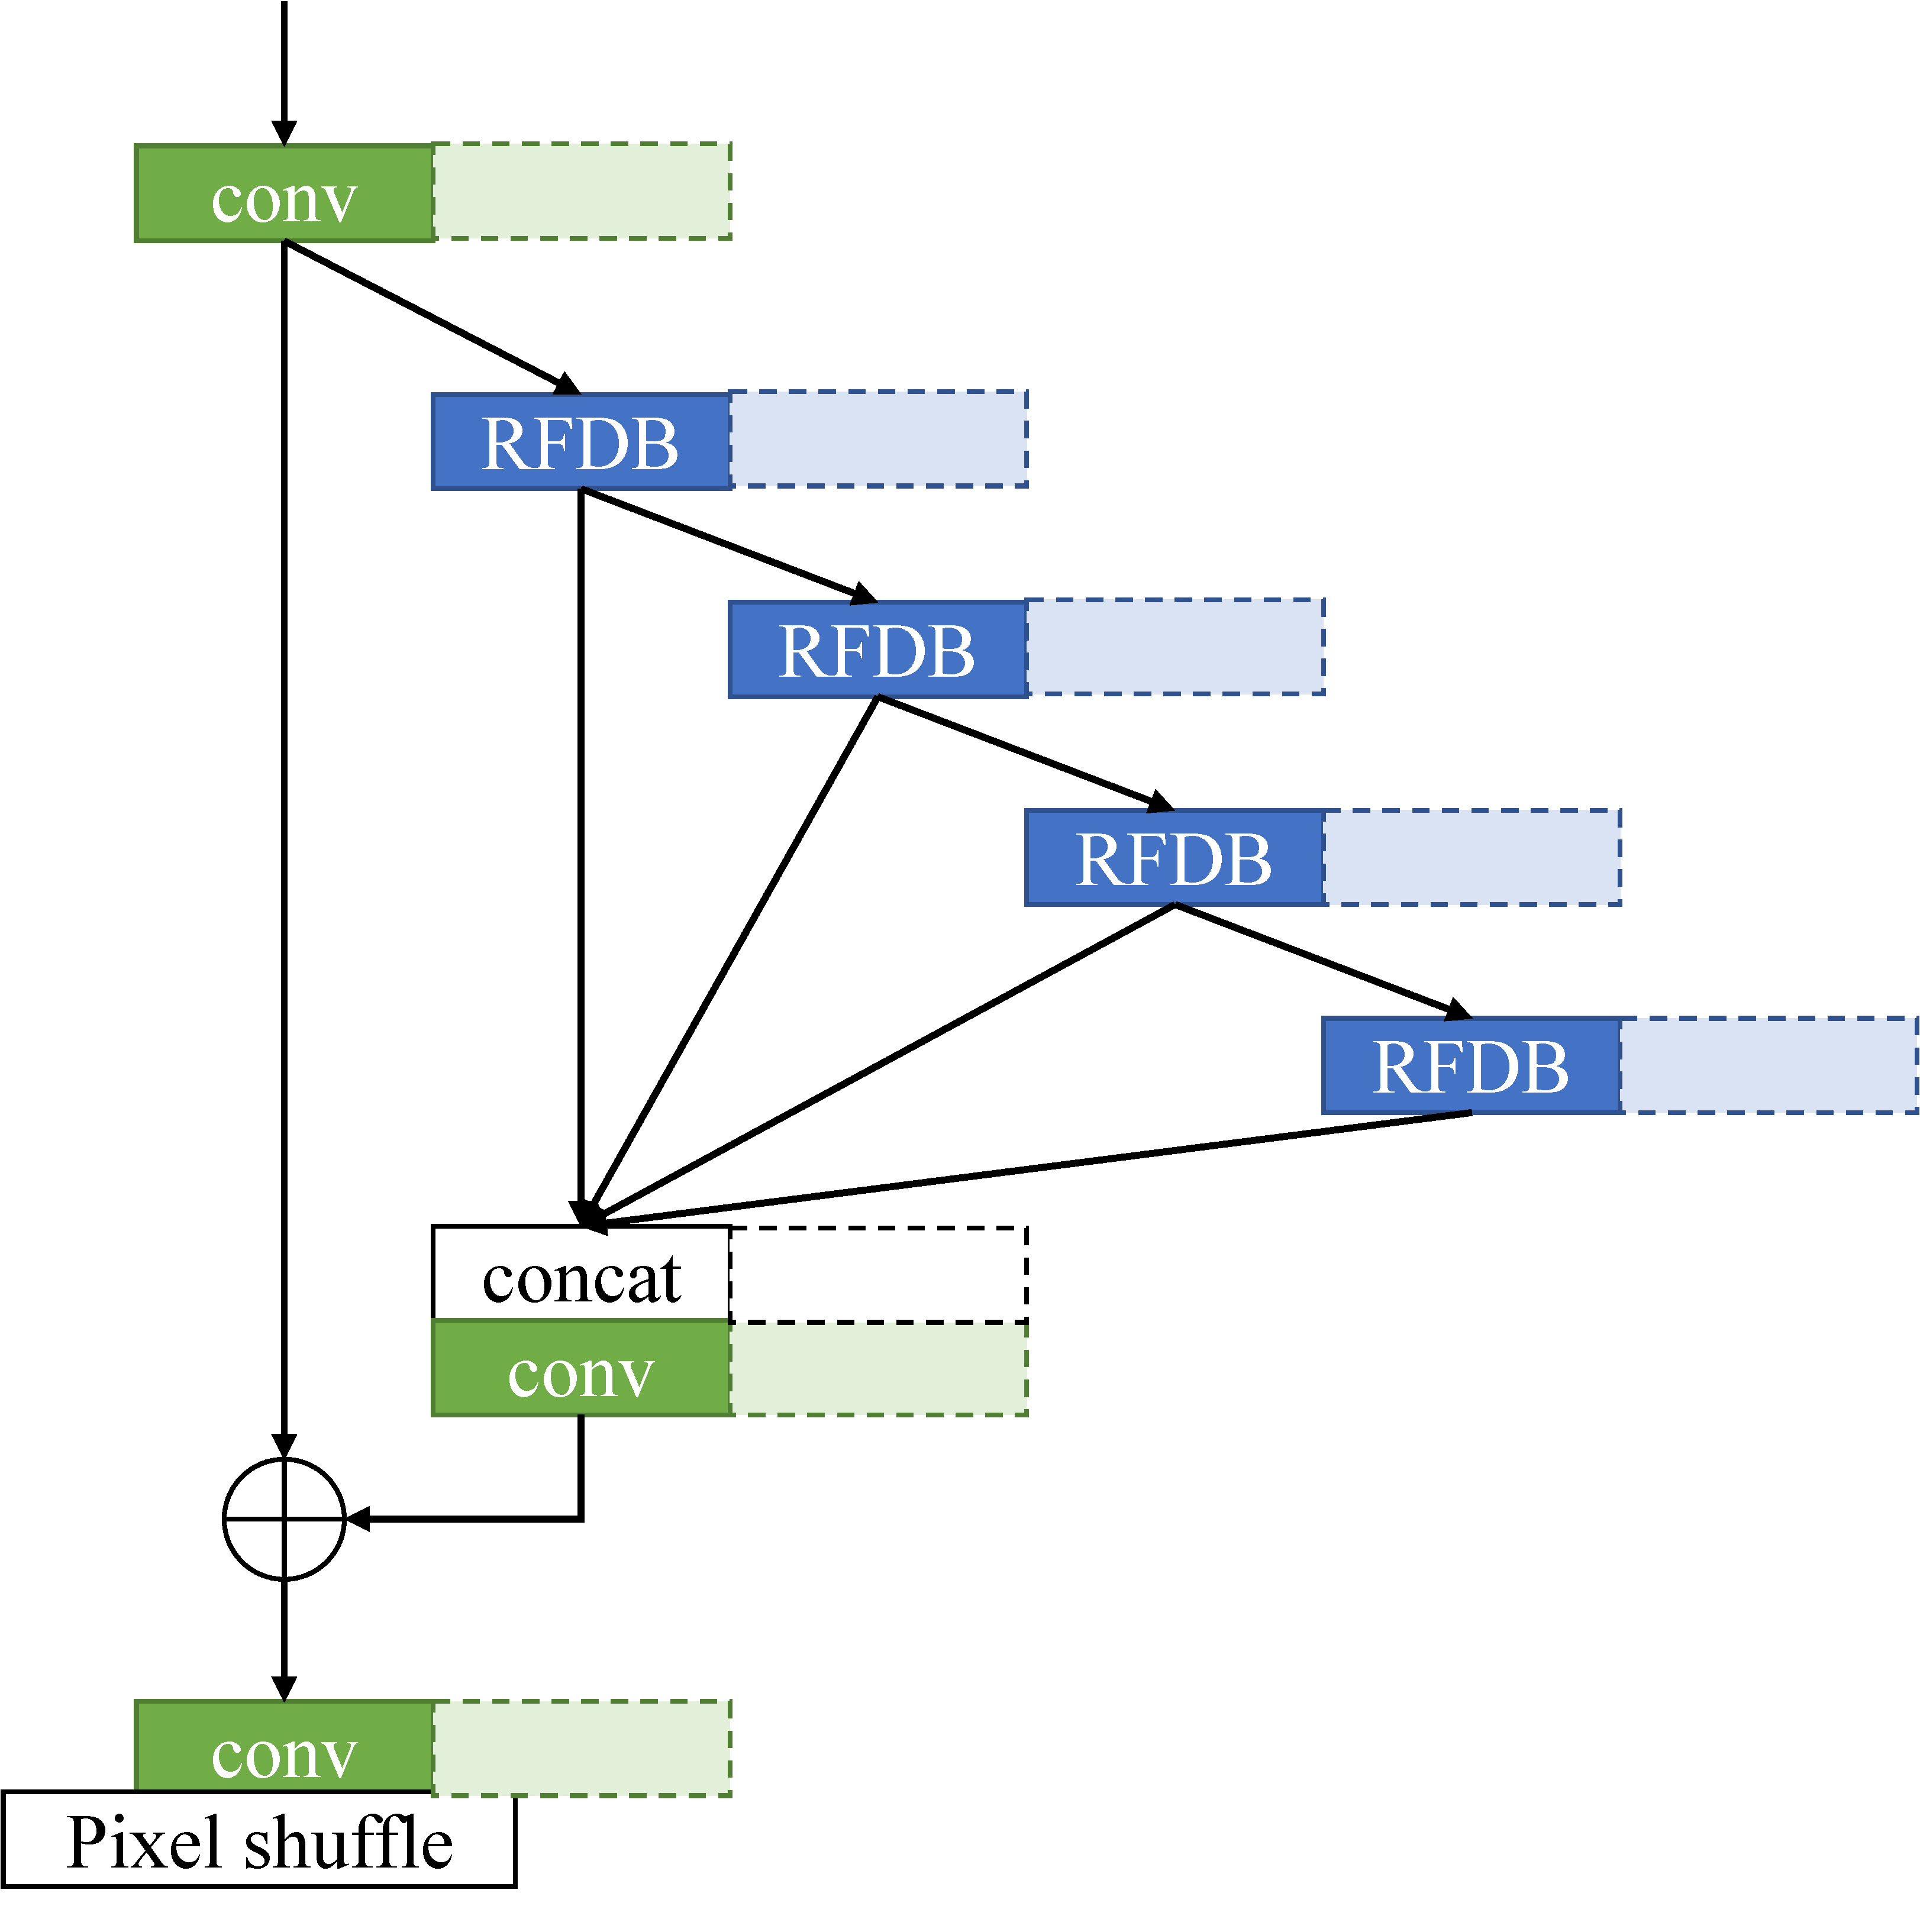
\includegraphics[width=\textwidth]{../expand.pdf}
        \caption{Expanding}
        \label{fig:Expanding}
    \end{subfigure}
    \begin{subfigure}[b]{0.49\linewidth}
		\centering
        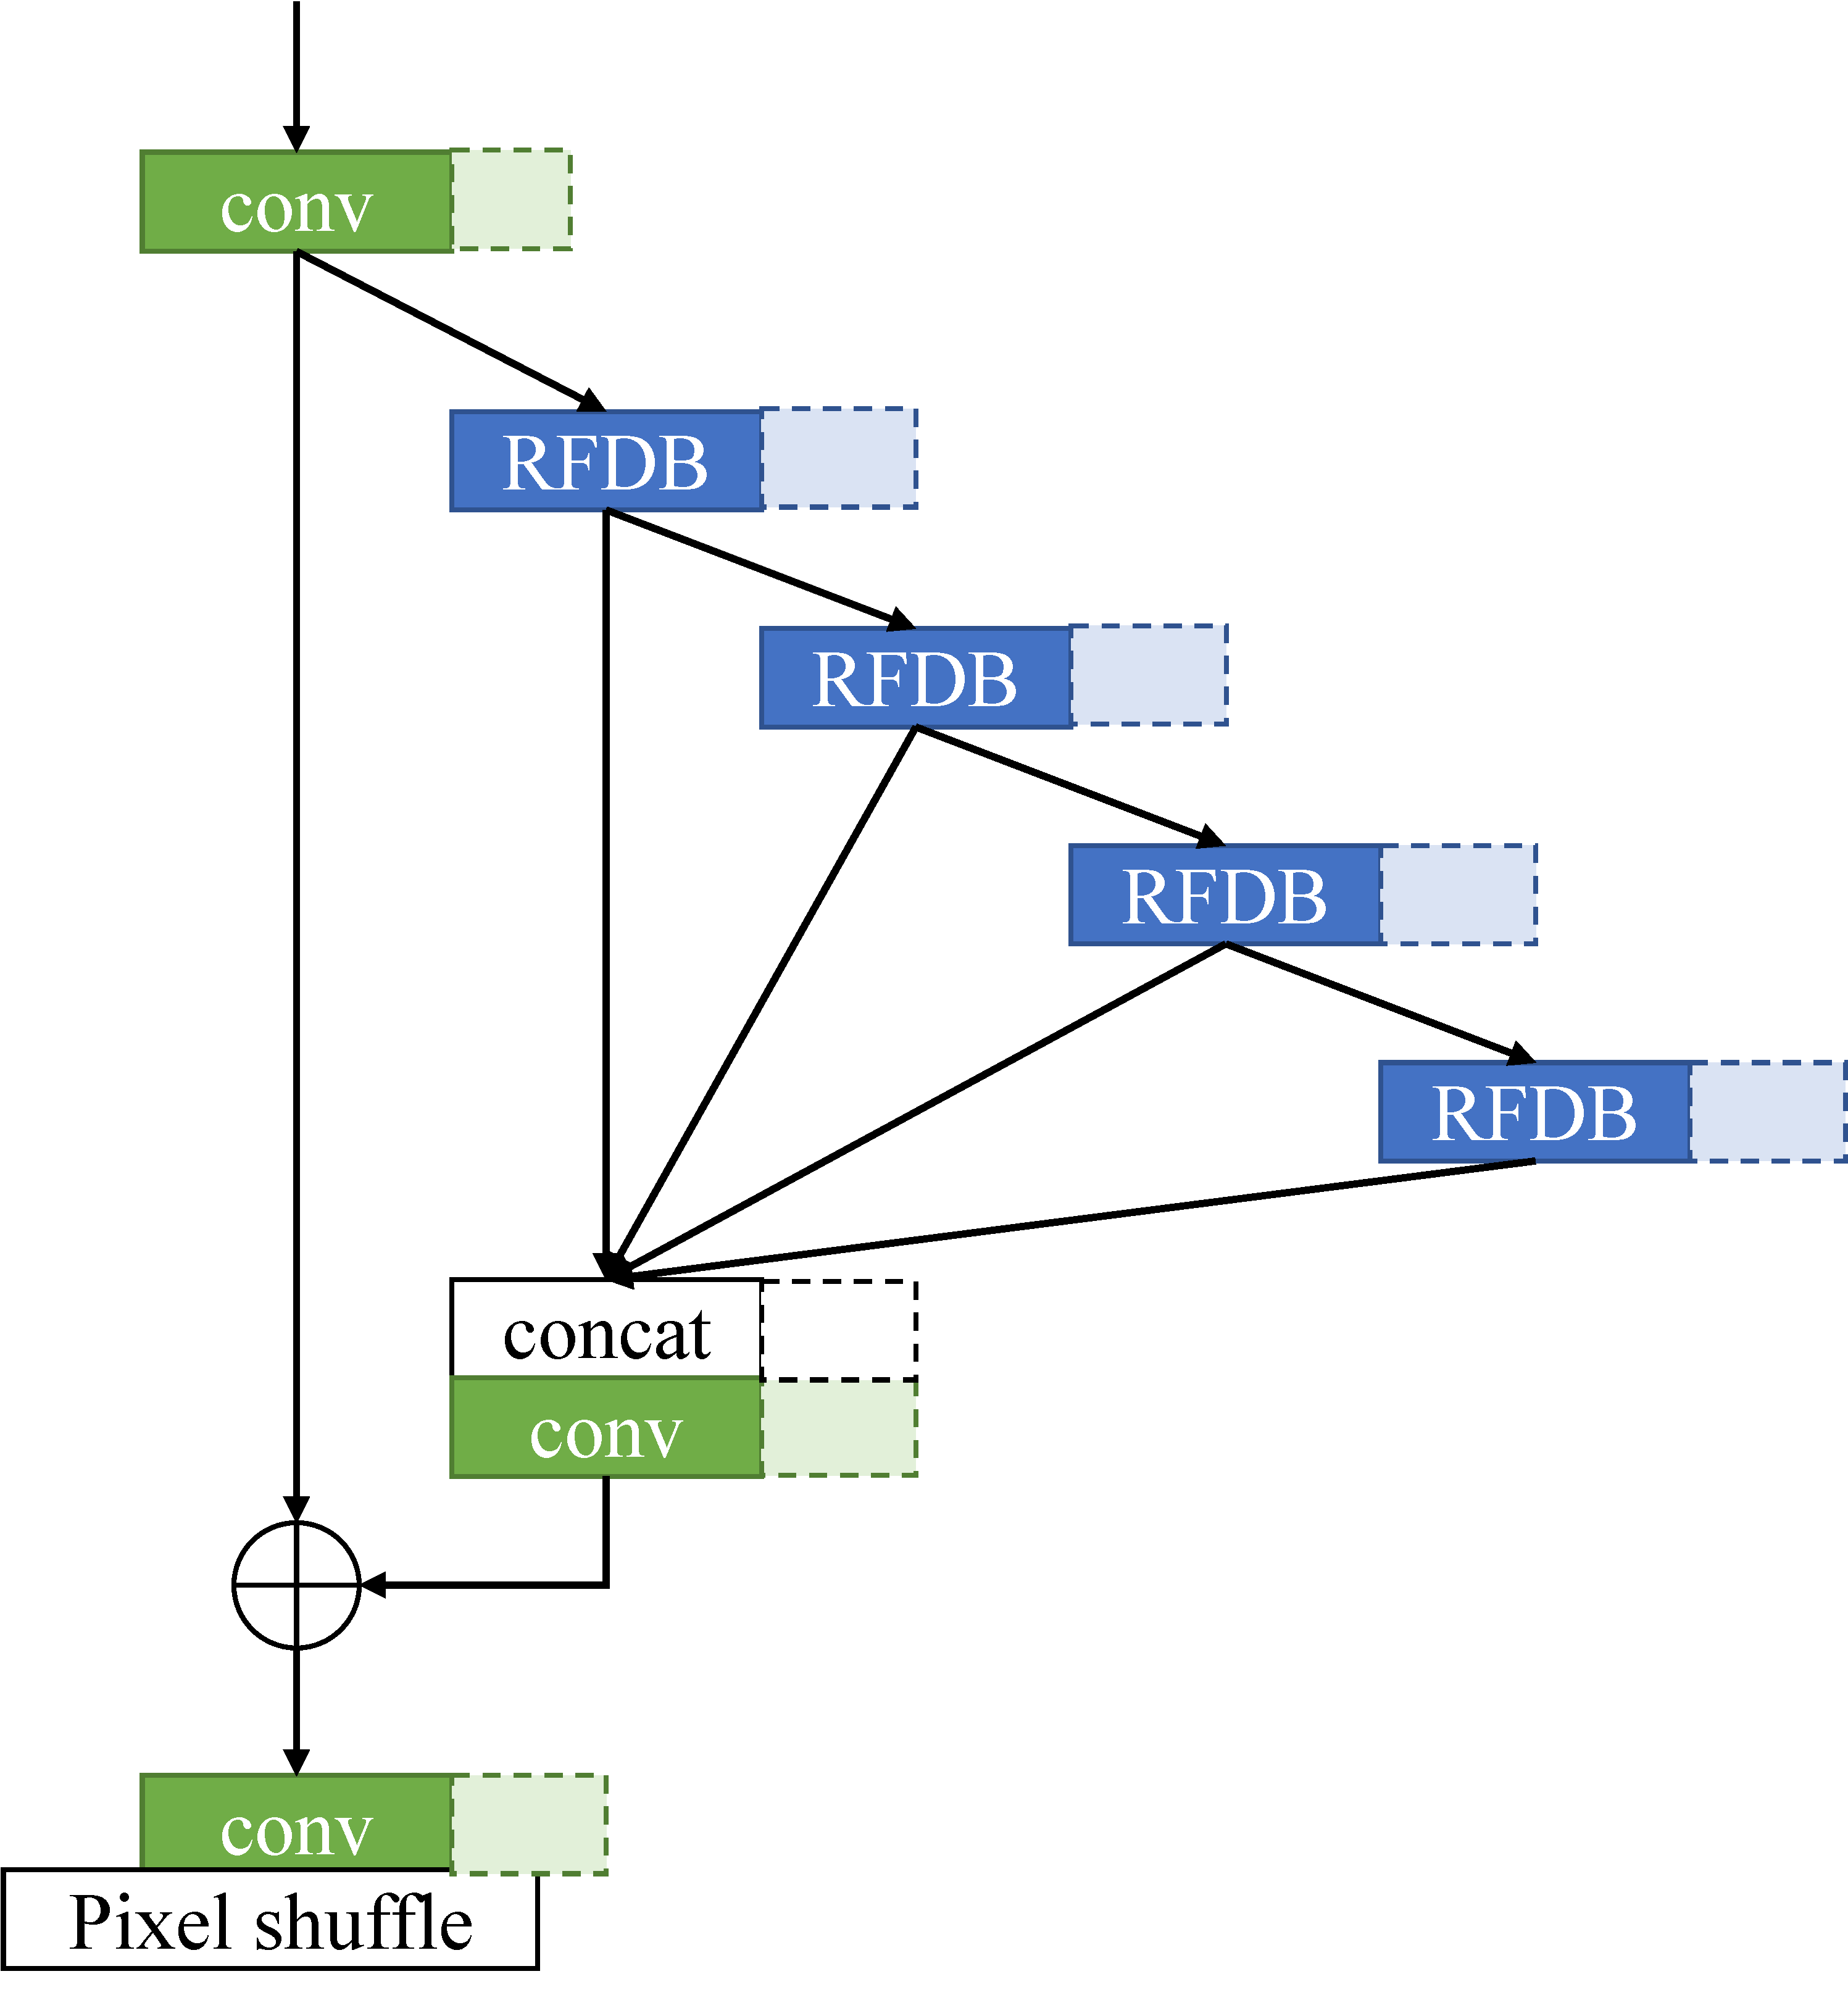
\includegraphics[width=\textwidth]{../shrink.pdf}
        \caption{Shrinking}
        \label{fig:Shrinking}
    \end{subfigure}
    \caption{Expanding and shrinking RFDN}
    \label{fig:PRFDN}
\end{figure*}

\subsection{Insights on designing efficient model.}
Lots of work focusing on designing efficient model to achieve SOTA performance on challenges year by year. A big problem under the phenomenon that collecting collect more data and create a new larger dataset for training a bigger and more powerful model is that we always need to update our model to adapt to the new dataset for learning more knowledge than before and also keep its efficiency which is always tedious.

Efficient insights are not easy to find and always ignored some important factors in the advanced computing platforms and due to good performance in theory but bad performance in reality which can happen on running MobileNet on different platforms.

We want to find a method that scaling an existing SOTA efficient model efficiently and effectively. By this way, we can just absorb achievements from efficient model design research and scale them to get a new SOTA in a new dataset.

We improve RFDN\cite{liu2020residual} model inspired on the "Train Big, Then Compress" theory proposed by \cite{li2020trainlarge} and proposed "Expand Big, Then Shrink" idea. On one hand, big model has more parameters than small model so that they can learn more knowledge from the dataset. If there is a new dataset larger than a traditional dataset which is the situation of LSDIR and DIV2K, the old SOTA model is not enough to learn new knowledge from the new large dataset, so that we need to expand it. On the other hand, a expanded model always has redundancy in computation, using compressing method to shrink it can make it efficient and without knowledge loss.

\subsection{Details}
We first expand all channels of operation in RFDN exclude pixelshuffle operation with 2x factor and then train it which is a big model training and achieved better results for its larger model capacity.
After training, a heavy compression followed.
We utilize a dynamic structure pruning method\cite{fang2023depgraph} to compress model and finetune it iteratively.

Prune and finetune description.

\subsection{Rethinking the complexity of expanding and shrinking.}

We used simple universal scaling methods to expand and shrink model structure but still achieving better accuracy-speed trade-off rather than the original model and the most of peers. On one hand, the way we used to expand model is based on width-multiplier which changed the width of all layers with a same scale. On the other hand, the way we used to shrink is a simple $\mathcal{L}1$ norm based pruner and also shrink all layers with a same scale. This result has proven the effectiveness and potency of the idea of "Expand and Shrink" scaling method.

%------------------------------------------------------------------------
\begin{figure*}[t]
    \begin{center}
    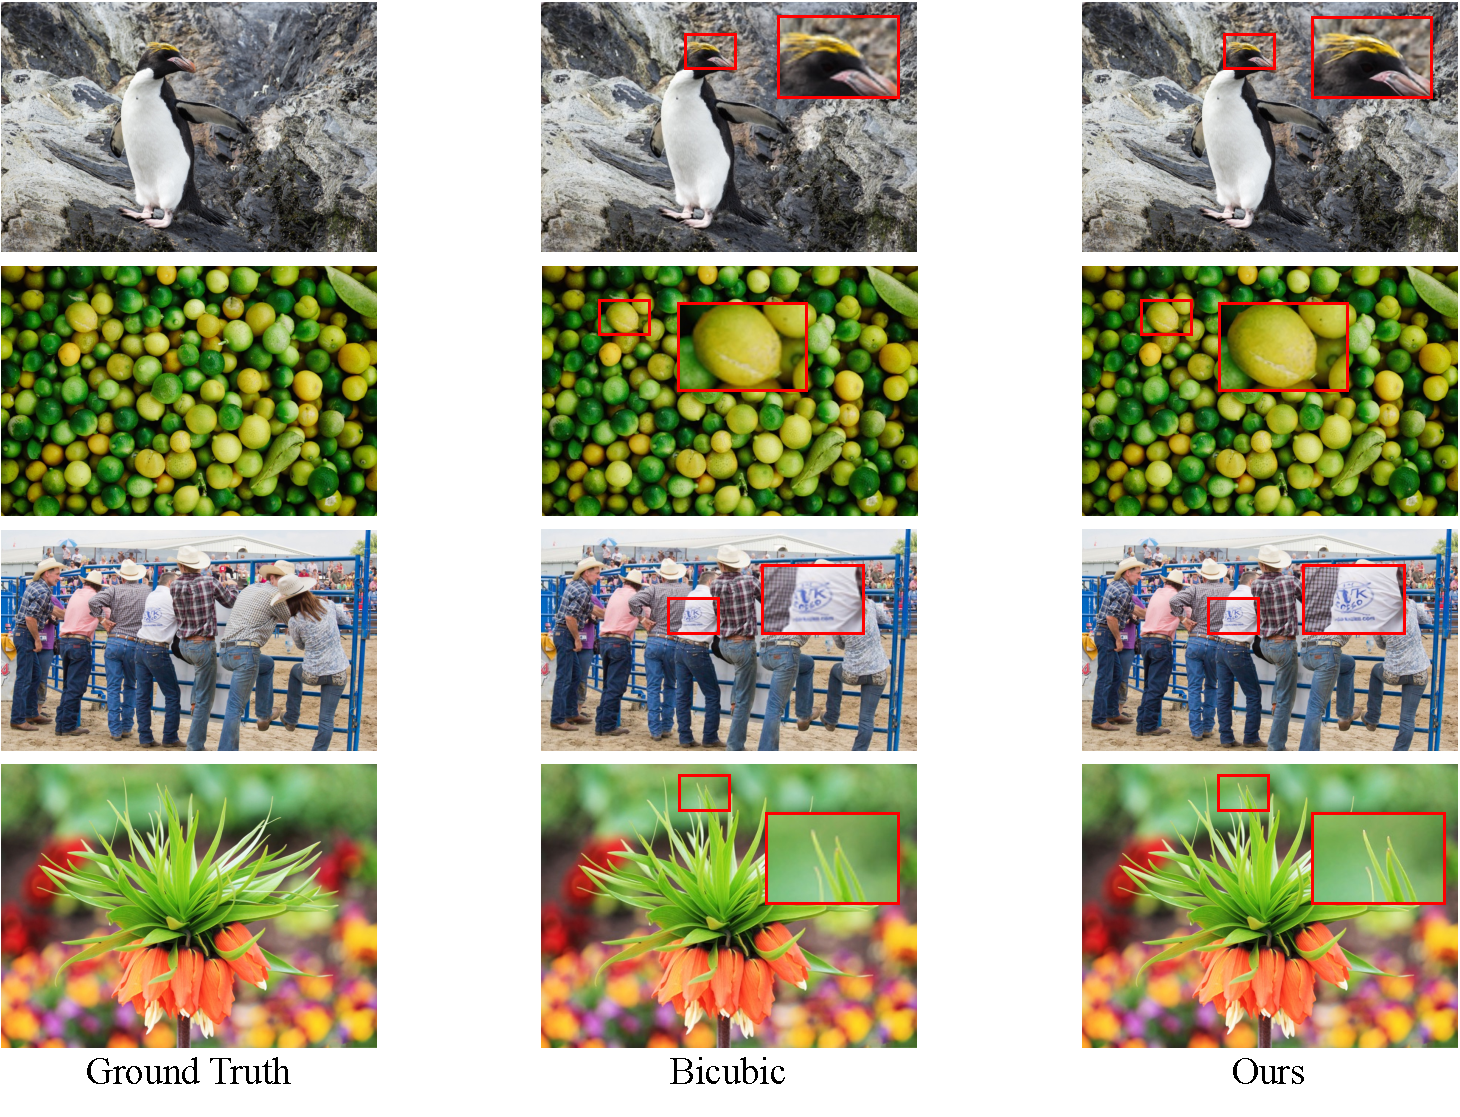
\includegraphics[width=\textwidth]{../x4result.pdf}
    \end{center}
    \caption{Comparison of image quality between our method and the bicubic method.}
    \label{fig:result}
\end{figure*}

\section{Experimental Evaluation}
\label{sec:exp}
In this section, we present the experimental evaluation of our proposed approach for image super-resolution. We first describe the experimental setup, including the datasets used, the hardware and software configurations, and the evaluation metrics. We then present the results of our experiments, which demonstrate the effectiveness of our approach.

\subsection{Experimental Setup}

\subsubsection{Datasets}
In this work, we use two widely used datasets in the field of super-resolution: DIV2K\cite{div2k} and LSDIR\cite{lilsdir} as the training datasets.

The DIV2K dataset is a widely used dataset for super-resolution tasks. It comprises 1000 images characterized by significantly higher resolution than those of the commonly referenced datasets. All the 1000 images are 2K resolution, that is they have 2K pixels on at least one of the axes(vertical or horizontal). All the images were processed using the same tools to $\times2$, $\times3$, and $\times4$ downscaling factors. The images cover a variety of scenes, including landscapes, portraits, and still-life compositions.

The LSDIR dataset proposes a large scale dataset for image restoration. It contains 84,991 high-quality training images and 250 validation images from the whole validation set. The dataset provides both high and low-resolution images for $\times2$, $\times3$, and $\times4$ downscaling factors.

For evaluation, we used Set5, Set14, BSDS100, and Urban100 datasets to verify the effectiveness of the image recovery quality of our method. These datasets contain a diverse range of images with different levels of complexity, making them suitable for evaluating the performance of super-resolution algorithms.

We evaluated our approach's computational efficiency using DIV2K dataset.


\subsubsection{Hardware and Software Configurations}
All experiments were conducted on a workstation equipped with an NVIDIA GeForce RTX 3070 GPU, 512GB of RAM, and an Intel(R) Xeon(R) Gold 6230R CPU. We used the Pytorch framework (version 1.13.0) for implementing and training our models. We used the Adam optimizer with a learning rate of 1e-5 and a batch size of 16 for training. We trained the model for 300 epochs on the DIV2K dataset and 300 epochs on the LSDIR dataset.

\subsubsection{Evaluation Metrics}
To evaluate the performance of our algorithm, we used two commonly used evaluation metrics: peak signal-to-noise ratio (PSNR) and structural similarity index (SSIM). Additionally, we report the validation time, test time, average time, model parameters, floating-point operations (FLOPs), activation volume, and memory consumption associated with our proposed algorithm. These metrics provide a comprehensive evaluation of our approach's effectiveness and computational efficiency.
\begin{table}[t]
  \centering
  \caption{Results of our computational efficiency on DIV2K dataset.}
  \resizebox{\linewidth}{!}{
  \begin{tabular}{cccccc}
    \toprule
    Ave Time[ms] & Params[M] &FLOPs[G] &Acts [M] & Mem[M] &Conv\\
    \midrule
    40.84&0.616&38.63&133.57&944.91&64\\
    \bottomrule
  \end{tabular}
  }
  \label{tab-runtime}
\end{table}

\begin{table}[t]
    \caption{Compared with the bicubic method, our method can effectively improve image quality.}
    \resizebox{\columnwidth}{!}
    {
        \begin{tabular}{|c|c|c|c|c|c|c|}
        \hline
        \multirow{2}{*}{Method} & \multirow{2}{*}{Scale} & \multirow{2}{*}{Params} & Set5  & Set14 & BSD100 & Urban100  \\
    \cline{4-7}          &       &       & PSNR/SSIM & PSNR/SSIM & PSNR/SSIM & PSNR/SSIM  \\
        \hline
        Bicubic & \multirow{2}[2]{*}{×4} & -     & 28.42/0.8104 & 26.00/0.7027 & 25.96/0.6675 & 23.14/0.6577  \\
        PRFDN (Ours) &       & 616K  & 30.20/0.8632 & 26.84/0.7444 & 26.24/0.7115 & 24.66/0.7662 \\
        \hline
        \end{tabular}%
    }
    \label{tab-quality}
\end{table}%
\subsection{Results}
Our approach achieves high PSNR and SSIM. Compared with the bicubic interpolation algorithm, we are able to get 4.3\% and 8.9\% improvement of PSNR and SSIM respectively. Figure\ref{fig:result} illustrates the comparison between our proposed super-resolution neural network model and conventional methods.The results demonstrate the effectiveness of our proposed super-resolution algorithm on high-resolution images. Table \ref{tab-quality} displays the quality performance of our approach methods on different datasets compared to other methods by PSNR and SSIM scores.

Furthermore, our approach achieves fast validation and test times, indicating its superior computational efficiency. Table \ref{tab-runtime} presents the performance of our proposed approach and state-of-the-art methods on the DIV2K dataset in terms of validation time, test time, average time, and memory consumption. Our approach achieves a fast average time with a result of 40.84ms on the DIV2K dataset. The test time and validation time are also significantly low. Specifically, our approach achieved a low test time of 33.33ms and a validation time of 48.35ms. Our approach's memory consumption is 944.91 MB.


\subsection{Discussion}
The results presented in this paper demonstrate the effectiveness and computational efficiency of our proposed super-resolution algorithm on two challenging datasets. Our method achieved high PSNR and SSIM scores on both DIV2K and LSDIR datasets, indicating that our approach can significantly enhance image resolution while preserving image details and textures.

Furthermore, our method showed remarkable computational efficiency, achieving a fast average time and low memory consumption compared to the baseline method. This is a crucial aspect for practical applications that require real-time super-resolution processing, such as video streaming and surveillance.

While our approach showed promising results, some limitations and potential directions for future research should be noted. We only trained our method on two datasets with a limited number of images, which could be investigated in future work.


%------------------------------------------------------------------------
\section{Conclusion}
\label{sec:conclud}

This paper presents a method for Efficient Image Super-Resolution (EISR) that addresses the need for computationally efficient and high-quality image production on mobile devices. We proposed an automatic model-scaling method, "Expand Big, Then Shrink," which expands and then shrinks an old SOTA model to adapt to a new and bigger dataset. This work contributes to the ongoing efforts in developing efficient models for SISR, which is crucial in various fields, including video gaming, video streaming, and mobile devices. Our proposed method provides a promising direction for future research and applications of EISR.


%%%%%%%%% REFERENCES
{\small
\bibliographystyle{ieee_fullname}
\bibliography{egbib}
}

\end{document}
